\documentclass[12pt]{article}
\usepackage[utf8]{inputenc}
\usepackage[T1]{fontenc}
\usepackage[brazil]{babel}
\usepackage{graphicx} % Required for inserting images
\usepackage[a4paper,left=3cm,right=2cm,top=3cm,bottom=2cm]{geometry} % Margens ABNT
\usepackage{setspace} % Espaçamento entre linhas
\usepackage{indentfirst}
\usepackage{subcaption}
\usepackage{threeparttable}
\onehalfspacing % Espaçamento 1,5 (padrão ABNT)

% ---------- PACOTES DE CITAÇÃO E BIBLIOGRAFIA (ABNT) ----------
\usepackage[alf,num=false,abnt-etal-cite=2,abnt-etal-list=0,abnt-etal-text=it]{abntex2cite}

% Dados do trabalho
\newcommand{\nomealuno}{Bruno Martins Valério Bomfim}
\newcommand{\titulotrabalho}{Uma proposta de implementação de ambiente virtual para prover recursos virtuais para disciplinas de computação}
\newcommand{\nomeorientador}{Prof. Dr. Fernando William Cruz}
\newcommand{\instituicao}{Faculdade de Ciências e Tecnologias em Engenharia/Universidade de Brasília — FCTE/UnB}
\newcommand{\programa}{Programa de Iniciação Científica}
\newcommand{\anorealizacao}{2026}

\begin{document}

% ---------- TÍTULO ----------
\begin{center}
    {\large \nomealuno}

    \vspace{0.3cm}

    {\Large \bfseries \titulotrabalho}

    \vspace{0.3cm}

    {\large \nomeorientador}

    \vspace{0.3cm}

    {\large \instituicao}

    \vspace{0.3cm}

    {\large \programa}

    \vspace{0.3cm}

    {\large \anorealizacao}
\end{center}

\vspace{1cm}

% ---------- RESUMO ----------
\section*{Resumo}

No contexto do Laboratório de Desenvolvimento de Sistemas (LDS) da Faculdade de Ciências e Tecnologias em Engenharia da Universidade de Brasília (FCTE/UnB), o compartilhamento do espaço físico e dos equipamentos entre diferentes disciplinas, turmas e horários constitui um problema recorrente. Este trabalho de Iniciação Científica tem como objetivo propor e prototipar a construção de um gêmeo digital do LDS na plataforma de metaverso descentralizado Decentraland, estabelecendo um canal de comunicação bidirecional entre o avatar do estudante e o equipamento físico correspondente. A pesquisa, de natureza aplicada e abordagem qualitativa e quantitativa, combinou um levantamento bibliográfico sistemático sobre metaverso educacional, gêmeos digitais e laboratórios virtuais/remotos com o desenvolvimento de uma prova de conceito. Os resultados demonstram a viabilidade técnica da sincronização bidirecional em tempo quase real entre o equipamento físico e sua representação virtual, corroborando as arquiteturas em camadas apontadas pela literatura como estratégia dominante para a implementação de gêmeos digitais em ambientes de metaverso, ao mesmo tempo em que contribuem para o preenchimento de uma lacuna identificada na literatura quanto à escassez de implementações educacionais que integrem, de forma avaliada, sincronização de gêmeos digitais, comunicação via IoT e interfaces imersivas. Conclui-se que a proposta é tecnicamente viável em escala reduzida, servindo de base para sua futura expansão ao contexto completo do LDS e para investigações posteriores sobre seu impacto pedagógico.
 
\vspace{0.5cm}
\noindent \textbf{Palavras-chave:} metaverso; gêmeo digital; laboratório remoto; Decentraland; braço robótico.

\newpage

% ---------- INTRODUÇÃO ----------
\section{Introdução}
\label{intro}

No contexto da FCTE/UnB, o Laboratório de Desenvolvimento de Sistemas (LDS) é utilizado por diversas disciplinas do curso de Engenharia de Software, o que gera um problema de compartilhamento do uso do espaço físico e dos equipamentos ali disponíveis entre turmas e horários distintos. Este projeto de Iniciação Científica tem como objetivo geral propor e prototipar a construção de um gêmeo digital do LDS na plataforma Decentraland, permitindo que estudantes explorem virtualmente o ambiente interno do laboratório e, principalmente, interajam com o gêmeo digital de um equipamento do laboratório, estabelecendo um canal de comunicação bidirecional entre o avatar e o dispositivo físico correspondente. Como prova de conceito para validação inicial dessa arquitetura, propõe-se o desenvolvimento de um gêmeo digital com sincronização bidirecional de um pequeno braço robótico controlado por microcontrolador (veja Subseção \ref{subsec:poc}).

Do ponto de vista da justificativa, acredita-se que a disponibilização do LDS em ambiente de metaverso pode incrementar significativamente a experiência de uso de laboratórios remotos, endereçando a barreira da distância física por meio de um serviço imersivo alternativo ao deslocamento presencial, com potencial ainda de viabilizar o uso inter-campi da infraestrutura. Espera-se, assim, que a imersão e a experimentação do LDS em metaverso gerem impacto pedagógico positivo, superando os limites físicos de espaço do laboratório e motivando investigações sobre a eficácia pedagógica do metaverso quando comparado a situações convencionais de uso presencial.

Este trabalho se insere como desdobramento do projeto UnBland, iniciado a partir do redesenho do repositório de recursos educacionais LMB para a plataforma Decentraland, e integra-se a um projeto de pesquisa mais amplo conduzido pela Profa. Dra. Germana Menezes da Nóbrega (CIC/UnB) e Prof. Dr. Fernando William Cruz (FCTE/UnB), que já reúne diversos trabalhos relacionados ao tema de metaverso educacional na UnB.

% ---------- REFERENCIAL TEÓRICO ----------
\section{Referencial Teórico}

\subsection{Metaverso, gêmeos digitais, laboratórios virtuais \& abordagens pedagógicas}
\label{subsec:referencial}

Para além de um caráter estritamente promocional, a literatura tende a definir o metaverso educacional como um ambiente persistente, multiusuário e compartilhado que integra atividades físicas e virtuais, tipicamente por meio de avatares, interfaces de realidade estendida (XR) e infraestruturas de dados ricas \cite{Wang2022Constructing, PenaRios2023Guest, Chen2026Metaverse}. Nesse sentido, a integração pretendida por diversos trabalhos não se resume à mera substituição de aulas presenciais por simulações em realidade virtual (RV) ou aumentada (RA); trata-se, antes, da constituição de um contínuo virtual-real, no qual os estudantes não apenas visualizam simulações, mas interagem com réplicas digitais de espaços, dispositivos ou sistemas capazes de espelhar o estado do mundo físico e, eventualmente, de controlá-lo \cite{Mitra2023Metaverse, Li2022When, Mihai2022Digital}.

Os gêmeos digitais desempenham papel central nessa integração, atuando como elo entre a pedagogia imersiva e os sistemas embarcados. São tipicamente definidos como réplicas digitais vinculadas a dados de ativos, processos ou sistemas físicos, capazes de sustentar monitoramento, predição e sincronização bidirecional, viabilizadas por sensoriamento IoT, computação de borda/nuvem e, mais recentemente, por modelos de inteligência artificial \cite{Li2022When, Mihai2022Digital, Yu2022BiDirectional, VanHuynh2022Edge}. A literatura converge para uma arquitetura em camadas amplamente recorrente entre as implementações de gêmeos digitais: sensores capturam o estado físico do ativo, o gêmeo digital representa esse estado no ambiente virtual, sistemas de borda/nuvem mantêm a sincronização de baixa latência entre as duas instâncias, e interfaces de RV/RA expõem o resultado ao usuário final \cite{Schroeder2021Methodology, Albalkhy2024Digital, Jagatheesaperumal2023SemanticAware}.

No que concerne aos laboratórios virtuais e remotos, a literatura os distingue de simulações puramente imersivas justamente pela presença dessa sincronização com equipamentos físicos reais. O projeto \textit{ReImagine Lab}, por exemplo, integra explicitamente laboratórios presenciais, virtuais e de controle remoto por meio de gêmeos digitais e RA \cite{Alsaleh2022ReImagine}, ao passo que o \textit{IM-MetaLAB} avança nessa direção ao empregar protocolos de Internet das Coisas (IoT) para que ações do estudante sobre um gêmeo fotorrealista de instrumentos de laboratório executem comandos sobre os instrumentos reais correspondentes \cite{Bonavolonta2025IMMetaLAB}. Uma revisão sistemática sobre laboratórios remotos estendidos, cobrindo o período de 2000 a 2022, reforça que essa integração entre virtualização e controle físico remoto constitui uma linha de pesquisa já consolidada, embora ainda concentrada em domínios específicos da engenharia \cite{Silva2023Extended}.

Do ponto de vista das abordagens pedagógicas, há razoável consenso entre revisões e estudos empíricos de que ambientes baseados em RV/RA e metaverso favorecem a imersão, a visualização, a colaboração e a prática segura de tarefas difíceis, perigosas ou de outra forma inacessíveis \cite{Kye2021Educational} \cite{Camilleri2023Metaverse}. Uma meta-análise sobre laboratórios virtuais na engenharia identificou efeito moderado sobre os resultados educacionais em geral e efeitos particularmente elevados sobre a motivação e o engajamento dos estudantes, ainda que os laboratórios virtuais não substituam integralmente a experiência prática presencial \cite{Li2024Effectiveness}. Resultado semelhante foi reportado por uma meta-análise voltada à formação de estudantes de enfermagem, na qual tecnologias imersivas melhoraram conhecimento, confiança e autoeficácia em comparação ao ensino tradicional, a despeito da heterogeneidade metodológica dos estudos primários \cite{Park2024Effects}. Uma revisão sistemática sobre RV e gamificação na educação corrobora esse padrão, associando a imersão a ganhos de motivação e engajamento em diferentes níveis de ensino \cite{Lampropoulos2024Virtual}.

É esse arcabouço conceitual -- o metaverso como continuum virtual-real, o gêmeo digital como mecanismo de sincronização bidirecional e as evidências de ganho pedagógico associado à imersão controlada -- que fundamenta a proposta de gêmeo digital do LDS descrita na Seção \ref{intro} e a prova de conceito detalhada na Subseção \ref{subsec:poc}.

\subsection{Trabalhos relacionados}

Este trabalho de iniciação científica é um desdobramento do projeto \textbf{UnBland}, principiado pelo artigo \textit{\lq\lq Redesenho e prototipagem de um repositório de recursos educacionais para metaverso\rq\rq} \cite{artigo_unbland}, no qual os autores propõem o redesenho e a prototipagem do repositório de recursos educacionais LMB (Lourdes Mattos Brasil) para a plataforma de metaverso descentralizado Decentraland, motivado pelo crescimento do interesse acadêmico em metaverso educacional e pela tradição de repositórios de objetos de aprendizagem ainda presos à navegação 2D.

Outro trabalho de conclusão de curso (TCC) desenvolvido pelo discente Thiago Vivan, do curso de Engenharia de Software da FCTE/UnB, entitulado \textit{\lq\lq Navegação Facilitada em Ambientes Universitários: Desenvolvimento de um Modelo 3D Interativo\rq\rq}, busca expandir o projeto UnBland, adicionando mais cenas no Decentraland com base na arquitetura real das edificações (Figuras \ref{fig:fga1} e \ref{fig:fga2}). Utilizando técnicas de modelagem no Blender e o Decentraland SDK, há a expectativa de que estes mapas sejam em breve adicionados ao contexto maior do UnBland.

\begin{figure}[htbp]
    \centering
    \begin{subfigure}[b]{0.45\textwidth}
        \centering
        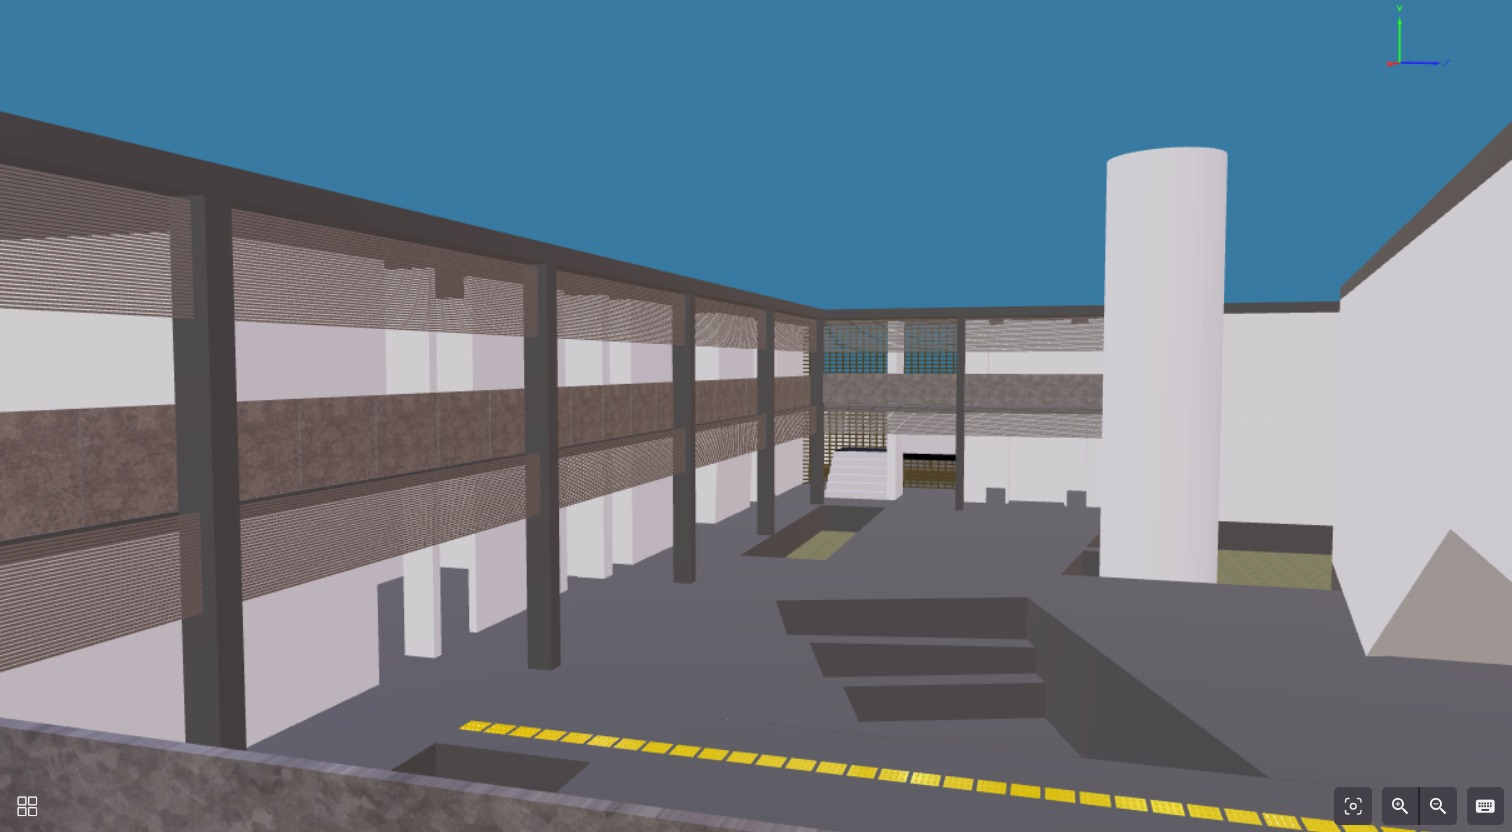
\includegraphics[width=\textwidth]{fga1.jpeg}
        \caption{Vista interior da UAC da FCTE/UnB.}
        \label{fig:fga1}
    \end{subfigure}
    \hfill
    \begin{subfigure}[b]{0.45\textwidth}
        \centering
        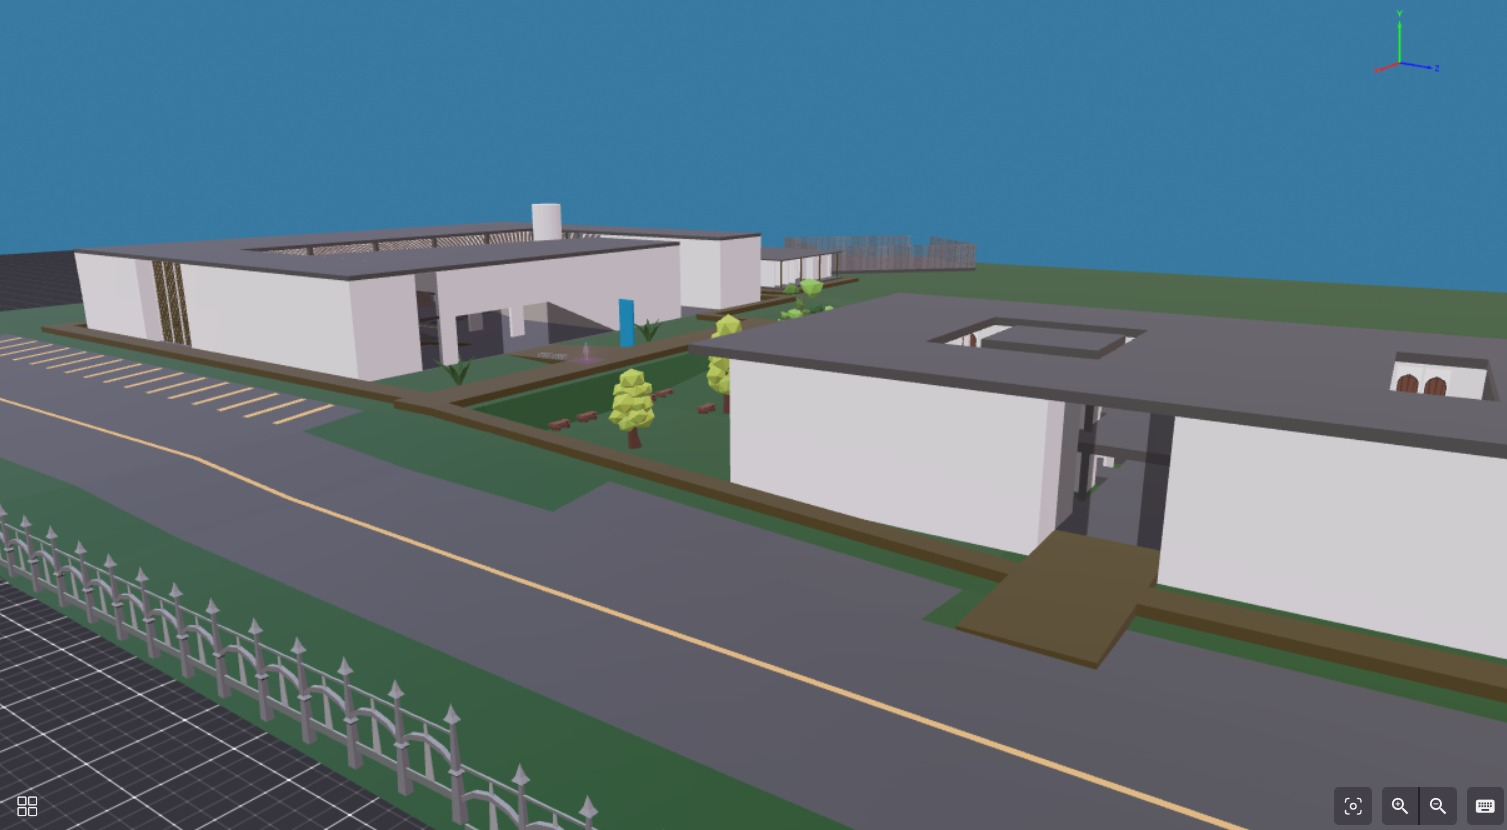
\includegraphics[width=\textwidth]{fga2.jpeg}
        \caption{Vista externa da FCTE/UnB.}
        \label{fig:fga2}
    \end{subfigure}
    \caption{Modelagem da FCTE/UnB no ambiente Decentraland. Fonte: Thiago Vivan, 2026.}
    \label{fig:fga}
\end{figure}

% ---------- METODOLOGIA ----------
\section{Metodologia}

Esta seção descreve os métodos que direcionaram as atividades realizadas neste projeto de iniciação científica. Apresenta-se também a classificação desta pesquisa e o respectivo levantamento bibliográfico, além de detalhamentos sobre a prova de conceito e o cronograma de atividades.

\subsection{Classificação da Pesquisa}
\label{test}

\citeonline[p.~33]{gerhardt_silveira} definem a pesquisa científica como \lq\lq o resultado de um inquérito ou exame minucioso, realizado com o objetivo de resolver um problema, recorrendo a procedimentos científicos\rq\rq. Seguindo a taxonomia proposta por estas autoras, é apresentada abaixo a classificação desta pesquisa quanto à \textbf{abordagem}, \textbf{natureza}, \textbf{objetivo} e \textbf{procedimentos}.

\subsubsection{Abordagem}

Esta pesquisa possui abordagem \textbf{qualitativa e quantitativa} \cite[p. ~33-36]{gerhardt_silveira}. O caráter \textbf{qualitativo} está relacionado à análise criteriosa de técnicas existentes na literatura científica para a resolução do problema proposto na seção \ref{intro}. De forma complementar, o aspecto \textbf{quantitativo} está relacionado à coleta e estudo de métricas concernentes à performance da solução proposta (veja \ref{levantamento}).

\subsubsection{Natureza}

Esta pesquisa possui natureza \textbf{aplicada} \cite[p. ~36-37]{gerhardt_silveira}, haja vista que almeja engendrar conhecimentos para a solução prática de um problema específico, a saber, o problema de compartilhamento dos laboratórios da FCTE/UnB.

\subsubsection{Objetivos}

Os objetivos deste estudo são \textbf{exploratórios} \cite[p.~37-38]{gerhardt_silveira}, envolvendo, assim, levantamento bibliográfico, e o estudo de caso do laboratório LDS da FCTE.

\subsubsection{Procedimentos}

Adotou-se a \textbf{pesquisa bibliográfica} \cite[p.~39]{gerhardt_silveira} cujo objetivo concentrou-se em identificar soluções propostas pela literatura científica para a implementação de gêmeos digitais em ambiente de realidade virtual ou aumentada. Ademais, a \textbf{pesquisa experimental} \cite[p.~38]{gerhardt_silveira} buscou construir uma solução para virtualização do laboratório LDS e a construção de uma prova de conceito no ambiente Decentraland.

\subsection{Levantamento Bibliográfico}
\label{levantamento}

Neste tópico são detalhados os procedimento adotados para a pesquisa bibliográfica para técnicas de virtualização de laboratórios para fins acadêmicos, e integrações com a Internet das Coisas (IoT).

\subsubsection{Strings de Busca}

Definiram-se strings de busca relacionadas ao tema em questão, submetidas a bases de dados como ACM Digital Library, Google Scholar, IEEE Xplore e Scopus. A Tabela \ref{tab:search_strings} apresenta uma síntese dos resultados obtidos, incluindo o número de resultados brutos e o número de trabalhos remanescentes após a aplicação dos critérios de seleção descritos na Seção \ref{criterios}. Foram considerados trabalhos publicados no período dos últimos 5 anos (2021-2026).

\begin{table}[h]
    \centering
    \caption{Strings de busca e resultados obtidos por base de dados. Fonte: Autor, 2026.}
    \begin{tabular}{| p{6cm} | p{1.65cm} | p{2.25cm} |}
        \hline
        \textbf{String de Busca} & \textbf{Base de Dados} & \textbf{Resultados Brutos} \\ \hline
        \lq\lq digital twin\rq\rq AND (\lq\lq remote lab*\rq\rq OR \lq\lq virtual lab*\rq\rq) & Google Scholar & 17500 \\ \hline
        \lq\lq digital twin\rq\rq AND (\lq\lq remote lab*\rq\rq OR \lq\lq virtual lab*\rq\rq) & IEEE Xplore & 138 \\ \hline
        metaverse AND education & Google Scholar & 30200 \\ \hline
        metaverse AND education & IEEE Xplore & 952 \\ \hline
        metaverse AND education & ACM & 1714 \\ \hline
        \lq\lq digital twin\rq\rq AND bidirectional & Google Scholar & 19000 \\ \hline
        \lq\lq digital twin\rq\rq AND bidirectional & IEEE Xplore & 468 \\ \hline
        \lq\lq digital twin\rq\rq AND bidirectional & ACM & 973 \\ \hline
        (\lq\lq virtual reality\rq\rq OR \lq\lq extended reality\rq\rq OR \lq\lq XR\rq\rq) AND (\lq\lq collaborative\rq\rq OR \lq\lq multi-user\rq\rq) AND (\lq\lq digital twin\rq\rq OR \lq\lq laboratory\rq\rq) & Google Scholar & 13600 \\ \hline
    \end{tabular}
    \label{tab:search_strings}
\end{table}

\subsubsection{Critérios de Seleção}
\label{criterios}

Os artigos identificados a partir das strings de busca foram avaliados segundo os critérios de inclusão e exclusão descritos a seguir.

\textbf{Critérios de inclusão} -- o artigo deve satisfazer ao menos um dos seguintes requisitos:

\begin{enumerate}
    \item Aborda arquiteturas ou mecanismos de sincronização entre um ambiente virtual (ou metaverso) e um equipamento físico real;
    \item Descreve implementações de gêmeos digitais aplicados a laboratórios educacionais ou de pesquisa;
    \item Reporta métricas de desempenho de rede (e.g., latência, \textit{throughput}, \textit{jitter}) relevantes para comunicação bidirecional em tempo real;
    \item Compara resultados de aprendizagem entre ambientes virtuais/remotos e laboratórios presenciais;
    \item Foi publicado em periódico ou conferência com revisão por pares, nos últimos dez anos.
\end{enumerate}

\textbf{Critérios de exclusão} -- o artigo será descartado caso se enquadre em pelo menos um dos itens abaixo:

\begin{enumerate}
    \item Trata de gêmeos digitais exclusivamente em contexto industrial ou de manufatura, sem relação com educação ou laboratórios remotos;
    \item Não possui texto completo disponível para acesso;
    \item É duplicata de um trabalho já identificado em outra base de dados;
    \item Consiste em resumo, pôster ou artigo com menos de quatro páginas;
    \item Emprega o termo ``metaverso'' de forma genérica ou mercadológica, sem contribuição técnica ou científica concreta.
\end{enumerate}

\subsection{Prova de Conceito}
\label{subsec:poc}

No contexto da engenharia de software, provas de conceito são ferramentas essenciais para demonstrar as capacidades e a adequação de um software, bem como demonstrar que um conceito é factível \cite[p.~1]{kottapalle_poc}. Nesse sentido, como prova de conceito para validar a viabilidade técnica da proposta, definiu-se o desenvolvimento de um gêmeo digital com sincronização bidirecional de um pequeno braço robótico, controlado por um microcontrolador ESP8266 e composto por quatro servomotores do tipo SG90. Essa prova de conceito antecede a aplicação da estratégia ao contexto completo do LDS, permitindo validar, em escala reduzida e controlada, os mecanismos de comunicação e sincronização que fundamentam a proposta descrita na Seção \ref{intro}.

Os resultados da prova de conceito são apresentados na seção \ref{res:poc}

% ---------- RESULTADOS E DISCUSSÃO ----------
\section{Resultados e Discussão}

\subsection{Da prova de conceito}
\label{res:poc}

A arquitetura da solução foi composta por três elementos principais: (i) o braço robótico físico, cujos servomotores foram controlados pelo ESP8266; (ii) um servidor de retransmissão (\textit{relay/bridge server}), desenvolvido na linguagem Go, responsável por intermediar a comunicação entre o equipamento físico e o ambiente virtual; e (iii) a cena correspondente no Decentraland, que representa o gêmeo digital do braço robótico. A comunicação entre a ESP8266 e o servidor de retransmissão ocorreu por meio do protocolo \textit{Message Queuing Telemetry Transport} (MQTT), amplamente utilizado em aplicações de Internet das Coisas (IoT) por seu baixo consumo de recursos e adequação a comunicações em tempo quase real. Tanto o servidor de retransmissão quanto a cena do Decentraland foram executados em uma máquina Linux local (\textit{on-premises}), o que permitiu maior controle sobre a infraestrutura durante a fase de prototipagem (Figura \ref{fig:system_design}).

\begin{figure}[htbp]
    \centering
    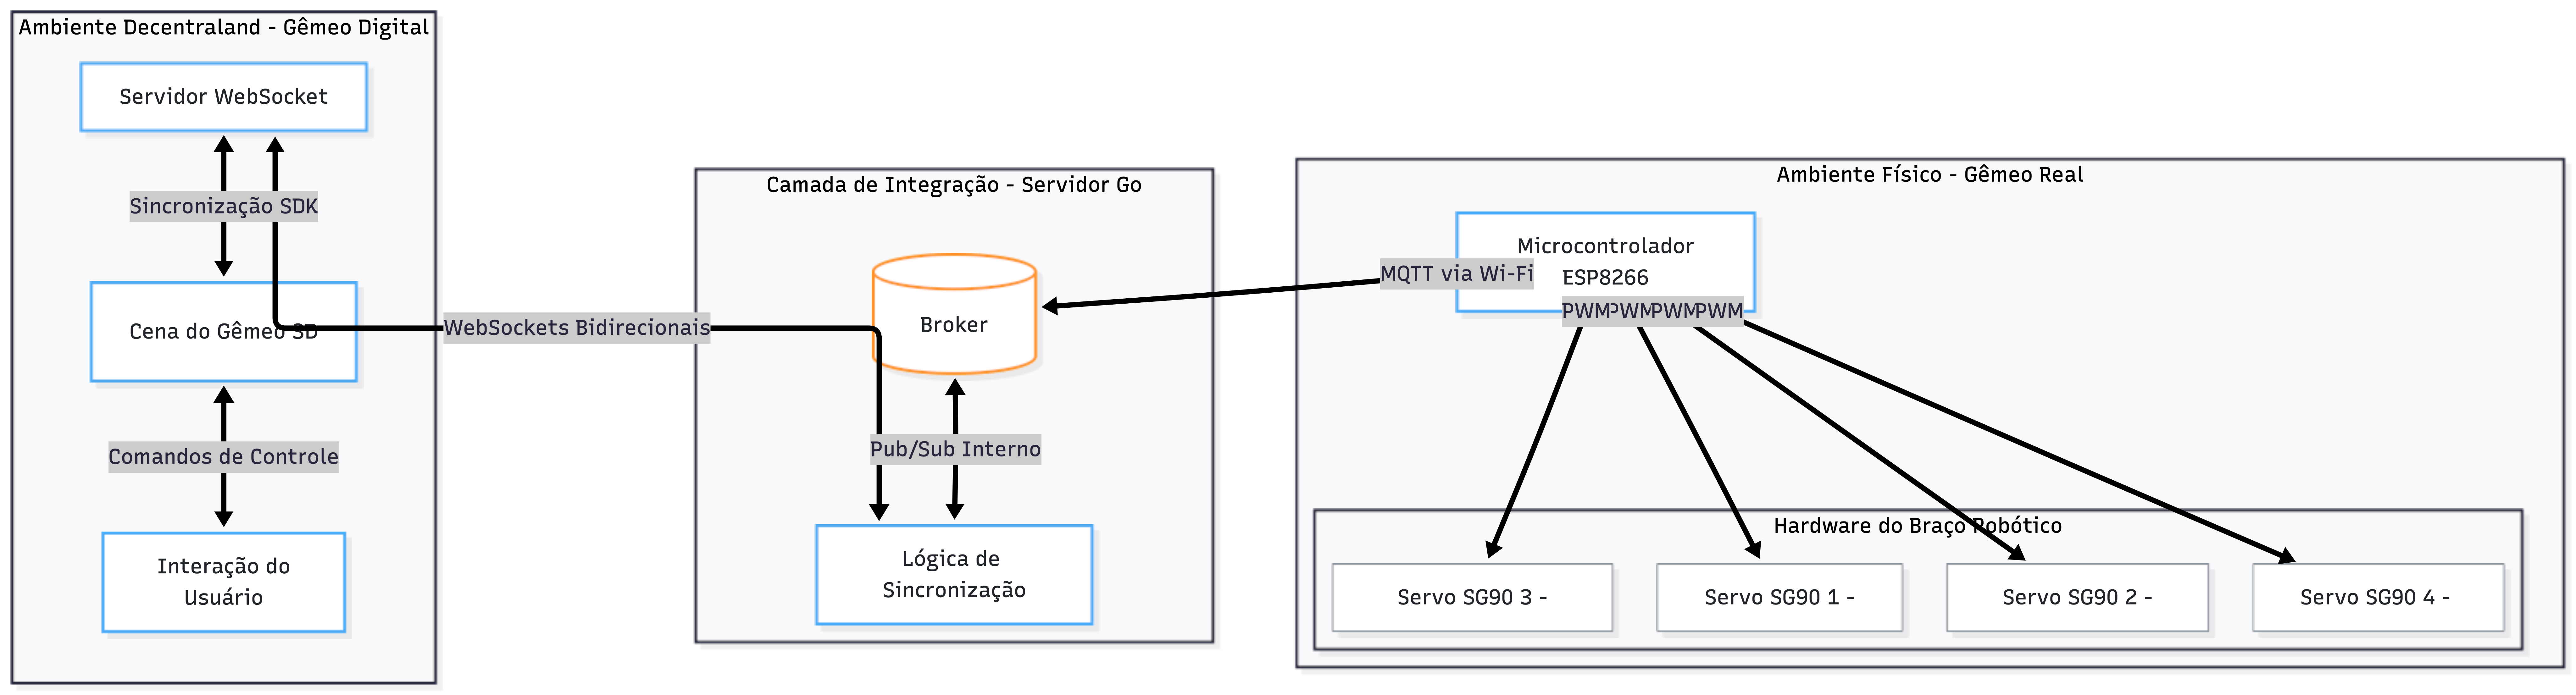
\includegraphics[width=0.75\textwidth]{poc.png}
    \caption{Arquitetura geral do sistema proposto. Fonte: Autor, 2026.}
    \label{fig:system_design}
\end{figure}

A sincronização proposta foi bidirecional: alterações realizadas no braço robótico físico — sejam elas comandadas manualmente ou por meio de um script de controle — deveriam refletir em tempo real na representação do braço no ambiente virtual, e, reciprocamente, comandos emitidos por um avatar no Decentraland devem ser transmitidos ao equipamento físico, provocando a movimentação correspondente dos servomotores. Para viabilizar múltiplos espectadores e/ou controladores simultâneos do gêmeo digital, adotou-se a estratégia de resolução de conflitos \textit{last command wins} (o último comando recebido prevalece), dispensando, assim, mecanismos mais complexos de fila ou bloqueio (\textit{locking}) de comandos concorrentes.

\begin{figure}[htbp]
    \centering
    \begin{subfigure}[b]{0.4\textwidth}
        \centering
        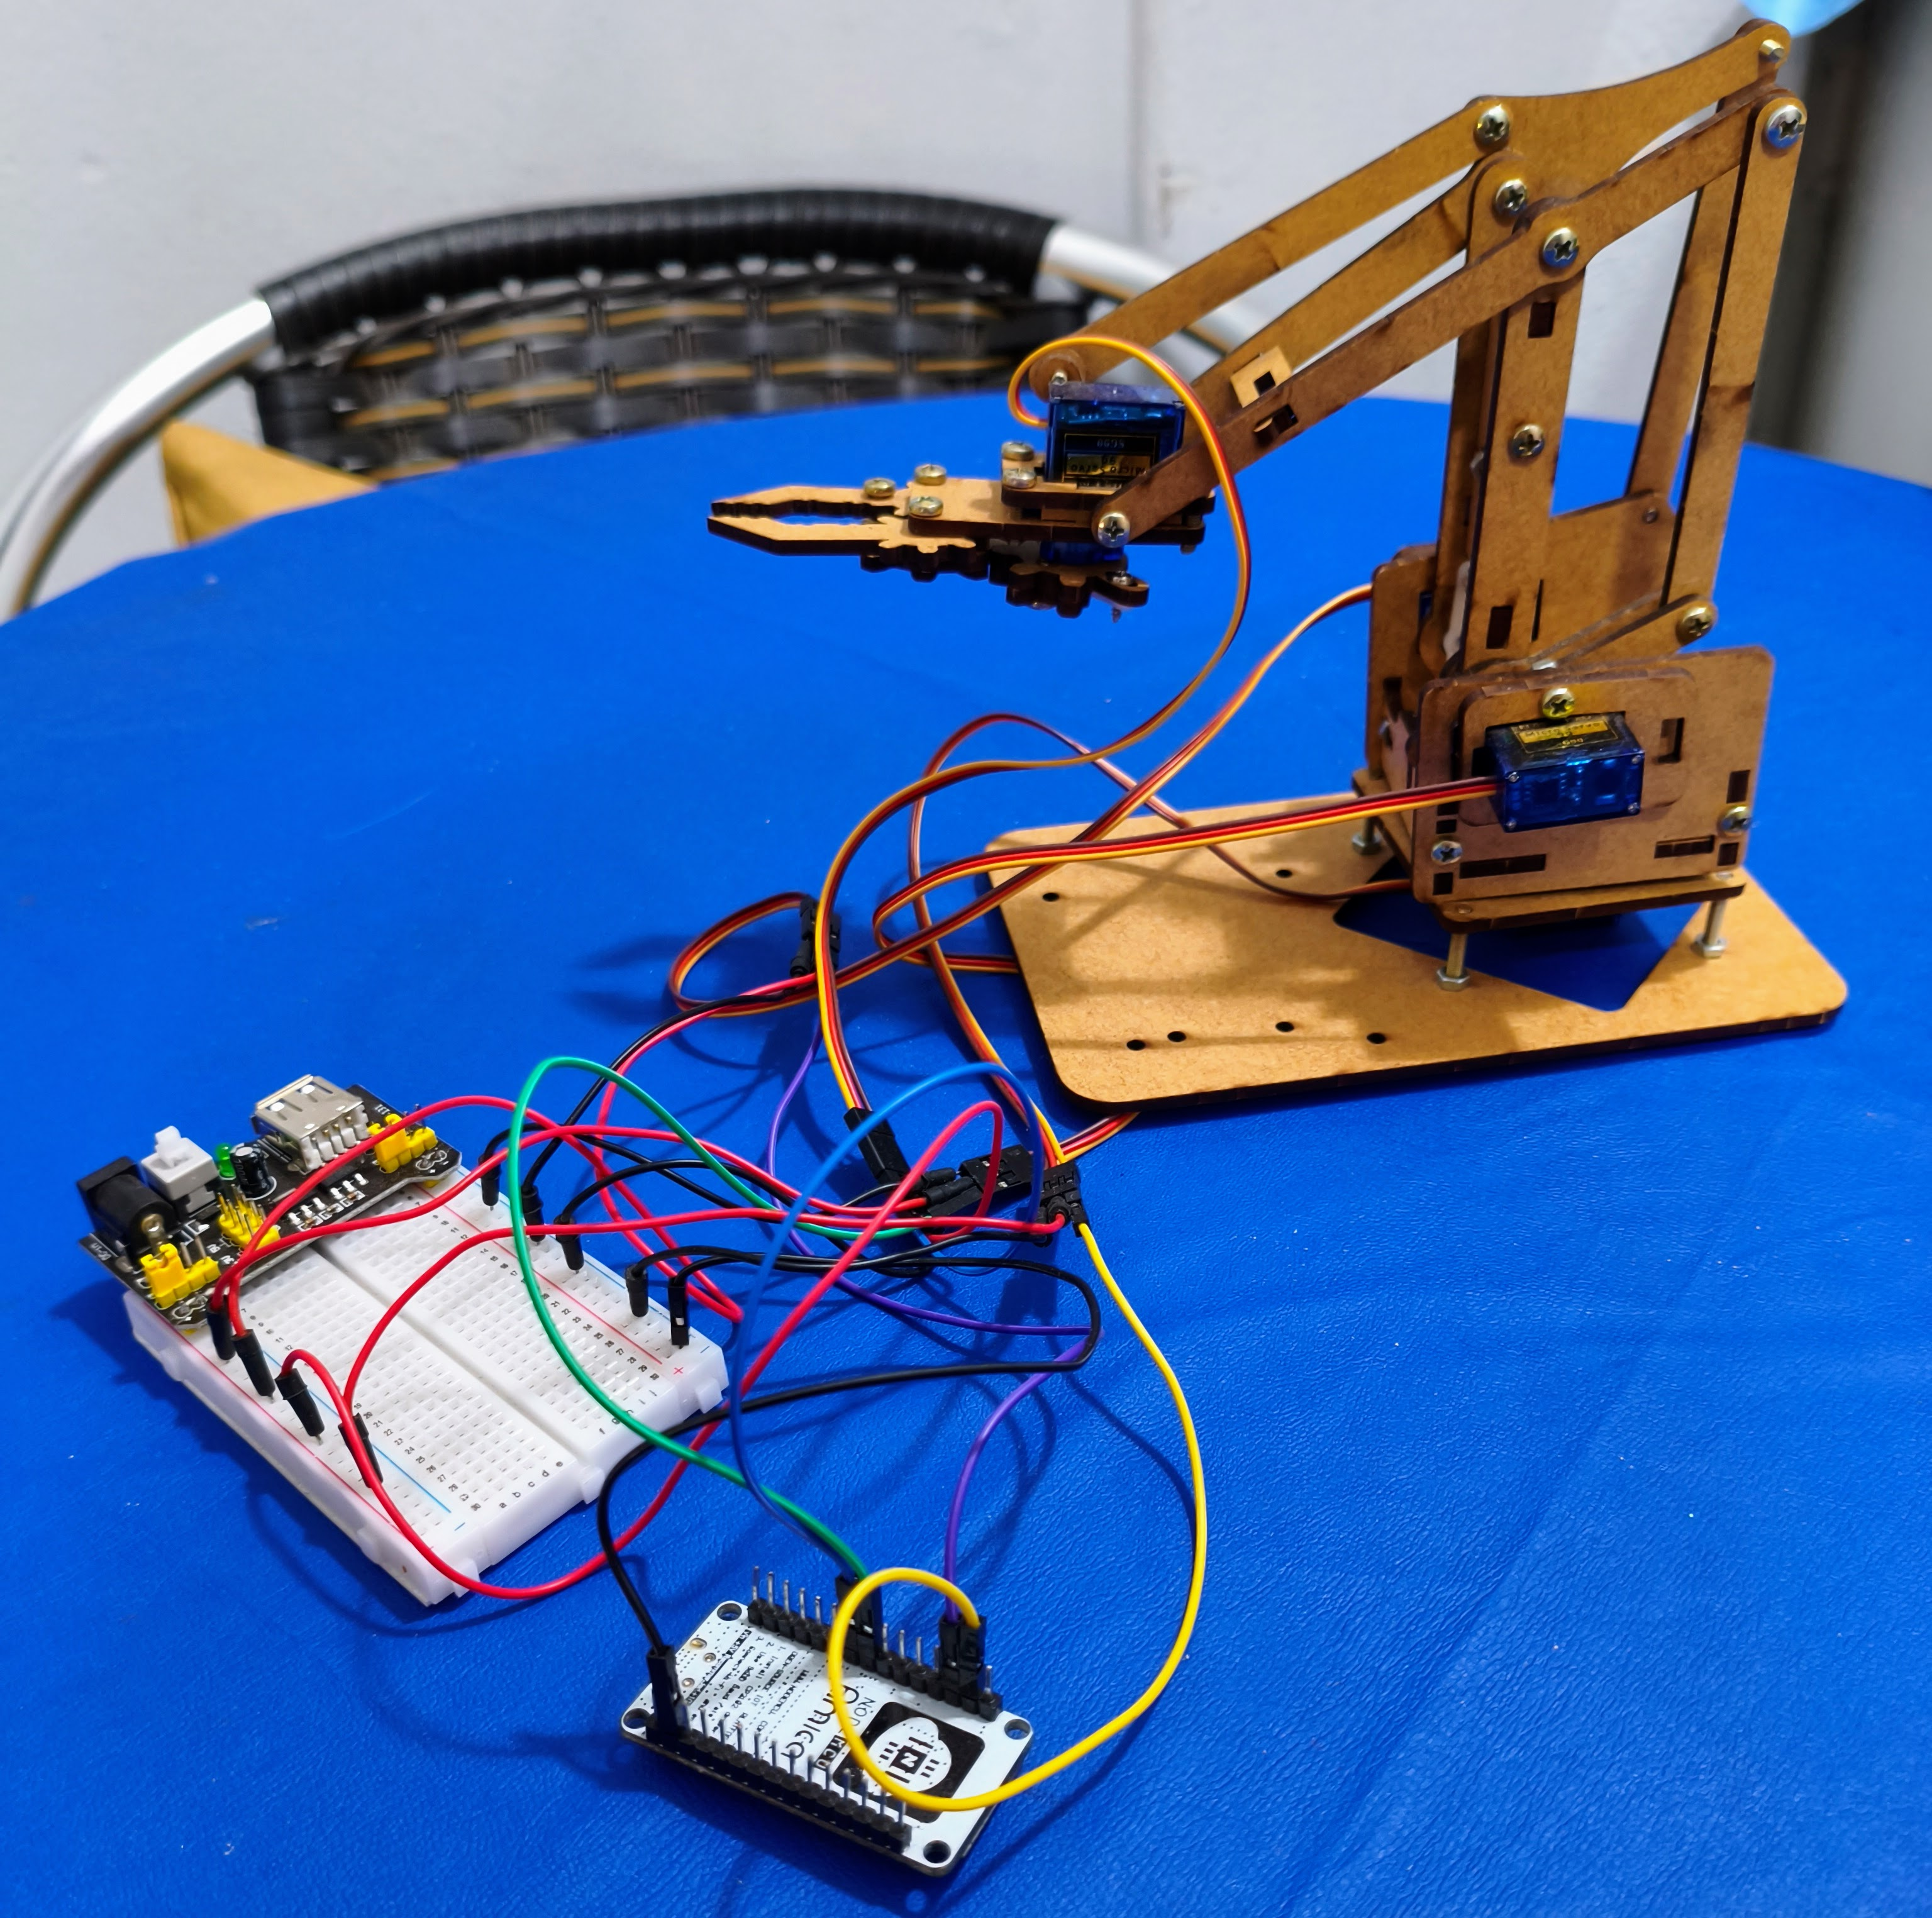
\includegraphics[width=\textwidth]{robot1.jpg}
        \caption{Mini-braço robótico produzido em MDF para a prova de conceito.}
        \label{fig:robot1}
    \end{subfigure}
    \hfill
    \begin{subfigure}[b]{0.5\textwidth}
        \centering
        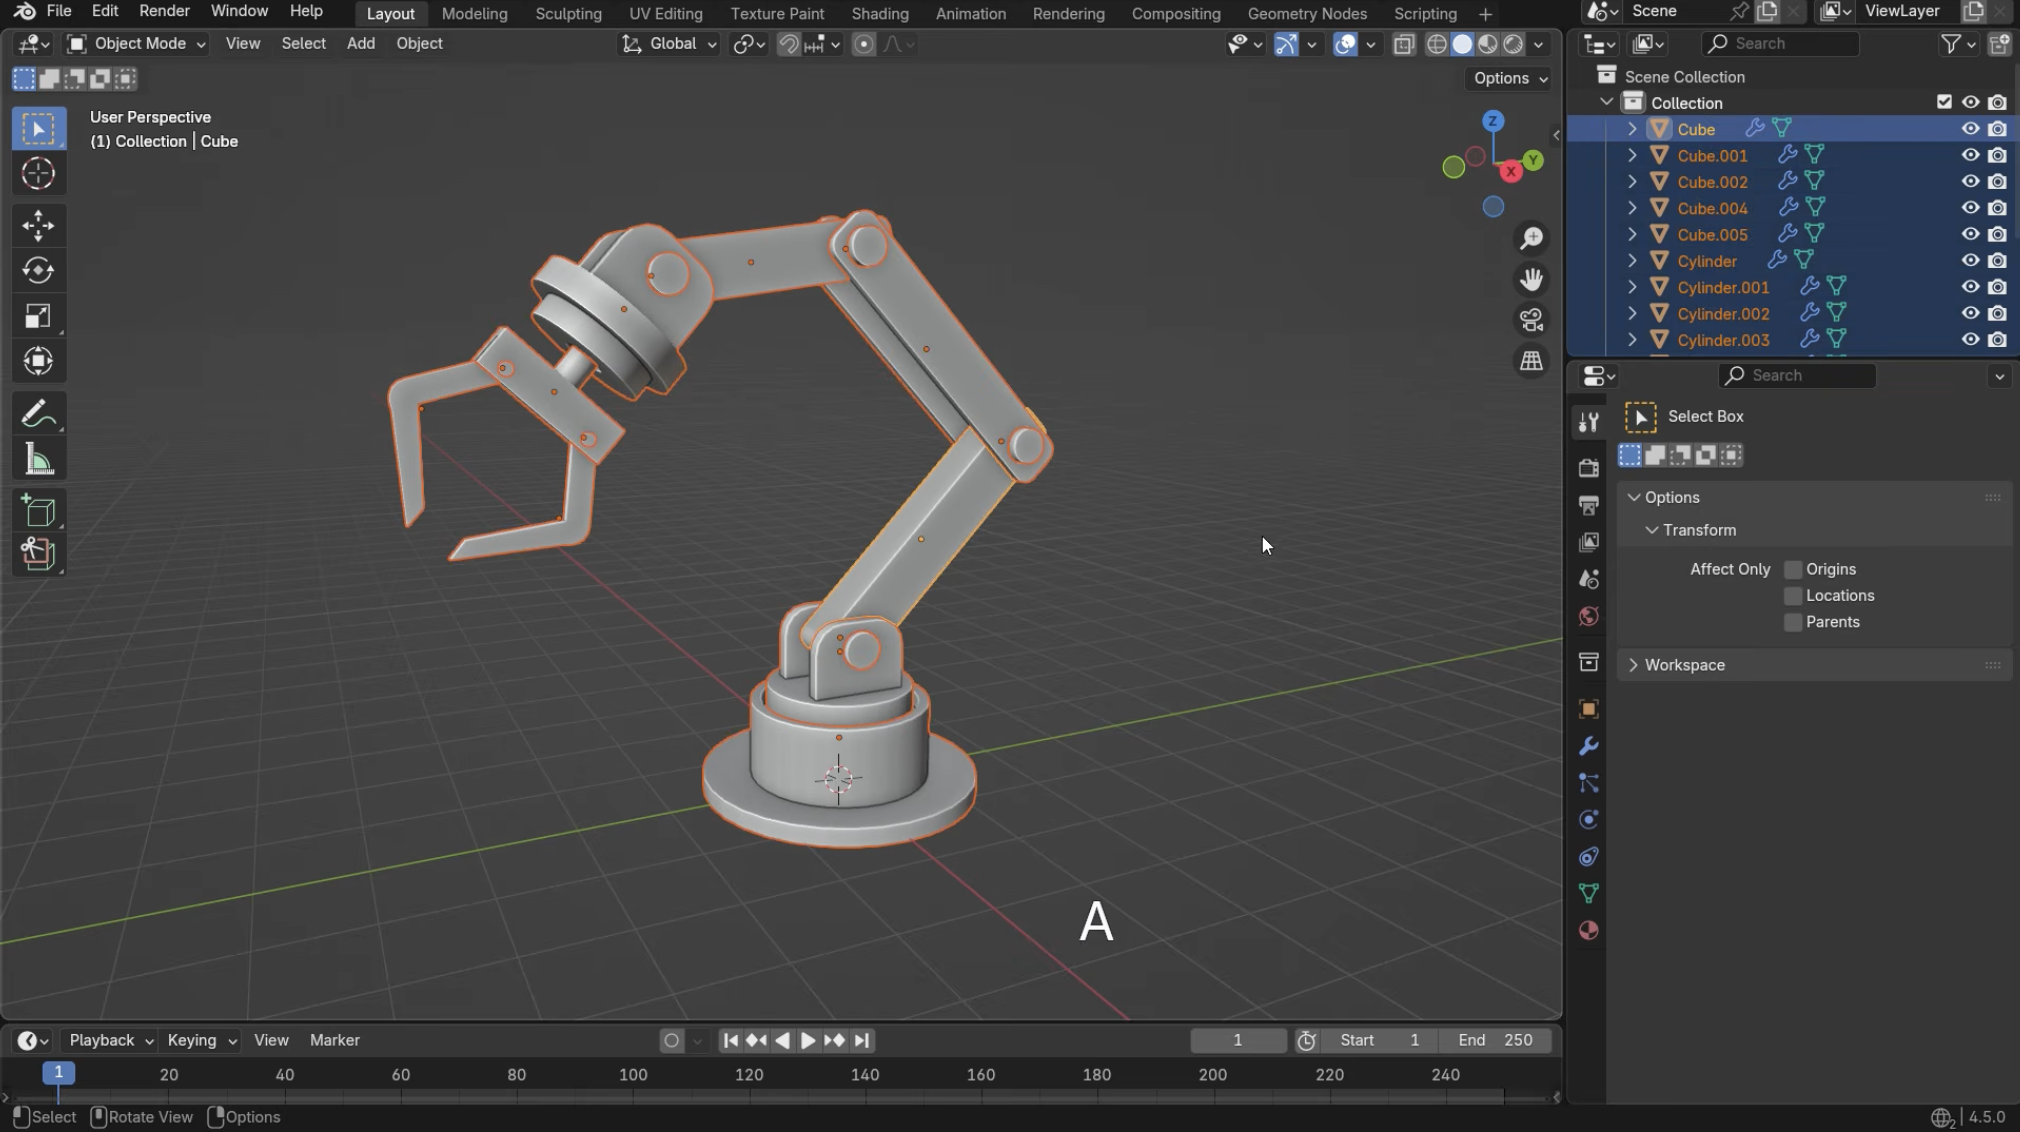
\includegraphics[width=\textwidth]{robot2.png}
        \caption{Modelagem do mini-braço robótico no Blender.}
        \label{fig:robot2}
    \end{subfigure}
    \caption{Modelagens física e virtual do mini-braço robótico. Fonte: Autor, 2026.}
    \label{fig:robot}
\end{figure}

\subsection{Da revisão de literatura}
\label{res:revisao}

A síntese dos trabalhos identificados segundo os critérios descritos na Seção \ref{levantamento} permite organizar as evidências em dois eixos complementares: um voltado à eficácia pedagógica da integração entre metaverso, laboratórios virtuais e gêmeos digitais, e outro voltado às estratégias técnicas de implementação de gêmeos digitais em ambientes de metaverso.

No primeiro eixo, há forte convergência entre revisões, meta-análises e estudos quase experimentais quanto ao fato de que sistemas integrados de RV/RA e metaverso melhoram o engajamento e os resultados de aprendizagem de curto prazo em diferentes áreas do conhecimento, como saúde, engenharia e ciências \cite{Li2024Effectiveness, Lampropoulos2024Virtual, Ibili2024Assessing}. Há também consenso crescente de que os gêmeos digitais constituem o mecanismo que transforma o metaverso de uma camada de visualização em um sistema de treinamento ciberfísico, ao manter a fidelidade de estado e viabilizar análise, predição e, por vezes, controle de ativos físicos \cite{Mitra2023Metaverse, Yang2025Live, Tu2024Architecture, Han2023A}. Por outro lado, a evidência é mais fraca quanto à eficácia em escala: diversas revisões relatam conceitos ainda fragmentados, projetos-piloto de pequeno porte, concentração regional dos estudos, padronização limitada e escassez de avaliação de longo prazo, sobretudo em contextos de alto risco \cite{Onu2023Potential, Sripan2025MetaverseBased, Jiang2025Virtual, Chen2026Metaverse}. Soma-se a isso o achado de que maior imersão nem sempre é desejável, podendo introduzir carga cognitiva extrínseca para estudantes iniciantes ou reduzir a usabilidade e o conforto em determinados contextos \cite{Poupard2024A}.

No segundo eixo, a literatura converge fortemente para arquiteturas em camadas como estratégia dominante, combinando sensoriamento físico, comunicação de dados, computação de borda/nuvem, modelos de simulação e interfaces de interação do usuário \cite{Schroeder2021Methodology, Albalkhy2024Digital, Yu2022BiDirectional}. Destaca-se, ainda, que a sincronização em tempo (quase) real é tratada como o principal gargalo técnico das implementações, sendo comum o emprego de estratégias de resolução de conflitos, de agendamento de atualizações e de predição de estado para preservar a fidelidade do gêmeo sem exaurir os recursos de rede e de computação disponíveis \cite{Liang2024Multiple, VanHuynh2022Edge}. A inteligência artificial é crescentemente incorporada a essas arquiteturas para viabilizar automação e escala, sendo empregada na construção e adaptação de modelos, na predição de estados futuros e na geração de conteúdo tridimensional \cite{Sajadieh2025From, Jamshidi2024An, Ahmed2025A}.

A lacuna mais evidente identificada na revisão é o descompasso entre a abundância de propostas arquiteturais conceituais e a escassez de implementações educacionais rigorosas que integrem, simultaneamente, interfaces de RV/RA, colaboração persistente multiusuário, sincronização de gêmeos digitais e sistemas de IoT embarcados em um único ambiente de aprendizagem avaliado empiricamente \cite{Xiao2025Industrial, Tu2024Architecture, Popov2024MetaverseBased}. É justamente nessa lacuna que se insere a prova de conceito descrita na Subseção \ref{res:poc}: ao articular um braço robótico físico controlado por microcontrolador, um servidor de retransmissão via protocolo MQTT e uma cena correspondente no ambiente Decentraland, a solução proposta reúne, em escala reduzida e controlada, os elementos de sincronização bidirecional, comunicação IoT e interface imersiva apontados pela literatura como necessários -- porém ainda pouco integrados e avaliados em conjunto -- para a consolidação de laboratórios educacionais ciberfísicos em ambiente de metaverso.

% ---------- CONSIDERAÇÕES FINAIS / CONCLUSÃO ----------
\section{Conclusão}
 
Este trabalho de Iniciação Científica partiu do problema de compartilhamento do Laboratório de Desenvolvimento de Sistemas (LDS) da FCTE/UnB entre as diferentes disciplinas, turmas e horários que dele fazem uso, e teve como objetivo geral propor e prototipar um gêmeo digital do LDS na plataforma Decentraland, capaz de estabelecer um canal de comunicação bidirecional entre o avatar do estudante e o equipamento físico correspondente do laboratório.
 
Para embasar essa proposta, realizou-se um levantamento bibliográfico sistemático (Seção \ref{levantamento}) sobre metaverso educacional, gêmeos digitais e laboratórios virtuais/remotos, cujos resultados (Subseção \ref{res:revisao}) confirmam que a integração entre ambientes imersivos e gêmeos digitais sincronizados por IoT tende a favorecer o engajamento, a motivação e, em menor grau, a aprendizagem de curto prazo dos estudantes, ao mesmo tempo em que revelam uma lacuna relevante: a escassez de implementações educacionais que integrem, em um único ambiente avaliado empiricamente, sincronização bidirecional de gêmeos digitais, comunicação via IoT e interfaces imersivas de metaverso.
 
Como prova de conceito para validar, em escala reduzida e controlada, a viabilidade técnica da arquitetura proposta, desenvolveu-se um gêmeo digital com sincronização bidirecional de um pequeno braço robótico controlado por um microcontrolador ESP8266 (Subseção \ref{res:poc}). Os resultados obtidos demonstram que é tecnicamente viável sincronizar, em tempo quase real, o estado de um equipamento físico com sua representação no Decentraland. Esse resultado corrobora, em escala reduzida, exatamente o tipo de arquitetura ciberfísica em camadas -- sensoriamento, comunicação, computação de borda e interface imersiva -- apontada pela literatura como estratégia dominante de implementação de gêmeos digitais (Subseção \ref{res:revisao}), ao mesmo tempo em que contribui para preencher a lacuna de implementações educacionais avaliadas nesse formato integrado.
 
É importante reconhecer, contudo, as limitações do presente estágio do trabalho. A prova de conceito restringiu-se a um único equipamento de pequena escala, executado em infraestrutura local, sem avaliação formal do impacto pedagógico da solução junto a estudantes. Como trabalhos futuros, sugere-se: (i) a expansão da prova de conceito para o ambiente completo do LDS, contemplando múltiplos equipamentos e cenários de uso concorrente; (ii) a condução de estudos de avaliação pedagógica que comparem, de forma controlada, o uso do gêmeo digital do LDS em metaverso com o uso convencional presencial do laboratório, conforme sugerido pela lacuna identificada na revisão de literatura; (iii) a mensuração formal de métricas de desempenho de rede sob condições realistas de uso simultâneo por múltiplas turmas; e (iv) a investigação de mecanismos de interoperabilidade entre plataformas de metaverso, de modo a viabilizar o uso inter-campi da infraestrutura, conforme originalmente motivado na Seção \ref{intro}. Por fim, este trabalho reforça e dá continuidade ao projeto UnBland e à agenda de pesquisa mais ampla sobre metaverso educacional conduzida na UnB, contribuindo com uma prova de conceito replicável de sincronização bidirecional entre ambientes físicos e virtuais.

% ---------- REFERÊNCIAS ----------
\newpage
\bibliography{references} 

\end{document}